\section{证明}
\subsection{特征~\ref{p1}证明}
\label{subsection:proof1}
\begin{proof}

不失一般性,假设用户 $a_i$对所有DApp的价值权
重为 $b_{i1}, b_{i2}, ..., b_{in}$。这些均为定值。
假设用户$a_i$对所有DApp的分贡献值分别为$\nr_{i1},...,\nr_{in}$,这些为可调整的变量。

用户$a_i$的优化目标为他所提供的总排名分,定义为
$$w_i = \sum_{j=1}^n b_{ij}\sqrt{\nr_{ij}}$$
根据柯西不等式可得
$$w_i = \sum_{j=1}^n b_{ij}\sqrt{\nr_{ij}} \leq (\sum_{j=1}^n b_{ij}^2)(\sum_{j=1}^n \nr_{ij}) \leq (\sum_{j=1}^n b_{ij}^2)\nr_i$$
上式最右边为定值。等号成立当且仅当
$$\frac{b_{i1}^2}{\nr_{i1}}=\frac{b_{i2}^2}{\nr_{i2}}=\cdots=\frac{b_{in}^2}{\nr_{in}}$$
故命题得证。

\end{proof}
\subsection{特征~\ref{p2}证明}
\label{subsection:proof2}
\begin{proof}
	 不失一般性,假设$d_1$开发者将其DApp拆分成2个DApp。对于章节~\ref{subsec:5.2}中第二种情形的正常用户$a_i$,即,拆分之前他对所有DApp的价值权重分别为$b_{i1},b_{i2},...,b_{in}$。拆分之后,假设$a_i$对于拆分出的$2$个DApp价值权重为$b'_{i1},b'_{i2}$。根据我们的假设有$b_{i1} \geq b'_{i1}+b'_{i2}$

	 我们接下来计算拆分之前的分贡献值。计$H_i = \sum_{j=2}^n b_{ij}^2$,根据特征~\ref{p1}的结论及合分比定理有
	 $$\frac{\nr_{i1}}{b_{i1}^2} = \frac{\sum_{j=1}^n \nr_{ij}}{\sum_{j=1}^n b_{ij}^2} = \frac{\nr_i}{b_{i1}^2+H_i}$$
	 故
	 $$\nr_{i1}=\frac{b_{i1}^2\nr_i}{b_{i1}^2+H_i}$$

     类似的可得到拆分之后$a_i$对拆分的第$t$个DApp的分贡献值为(定义为$\nr'_{it},t=1,2$)
	 $$\nr'_{it} =  \frac{b_{it}^{'2}\nr_i}{b_{i1}^{'2}+b_{i2}^{'2}+H_i}$$
	 注意到$b_{i1}^2 \geq (b‘_{i1}+b’_{i2})^2 >b_{i1}^{'2}+b_{i2}^{'2}$,可得
	 $$\nr_{i1} > \nr'_{i1}+\nr'_{i2}$$
	 上述分析了对于一个足够聪明的理性用户选择的分贡献值满足的条件。事实上,对于大部分普通用户,他们属于章节~\ref{subsec:5.2}中第一种情形,即,他们面对DApp拆分所采取的方式通常为简单的将原本投给拆分前的DApp的所有票分散开来。无论哪种情况,均有
	 	$$\nr_{i1} \geq \nr'_{i1}+\nr'_{i2}$$

	 定义$S'_1,S'_2$分别为$d_1$拆分之后的两个DApp的排名分,根据定义,有
	 $$S'_1 =  \sum_{i=1}^m \sqrt{\nr'_{i1}},~~~S'_2 =  \sum_{i=1}^m \sqrt{\nr'_{i2}},~~~S_1 = \sum_{i=1}^m \sqrt{\nr_{i1}}$$
	 定义$U'_1$为拆分之后$d_1$开发者从所有DApp中获得的奖励,则
	 $$U'_1=\frac{S_1^{'2}+S_2^{'2}}{S_1^{'2}+S_2^{'2}+\sum_{j=2}^n S_j^2} \lambda M,~~~U_1=\frac{S^2_1}{S_1^2+\sum_{j=2}^n S_j^2} \lambda M$$
	 注意到在固定$S_2,...,S_n$的情况下,
	 $$ U_1 \geq U'_1 \Leftrightarrow S_1^2 \geq S_1^{'2}+S_2^{'2}$$

	 所以,为了比较$d_1$开发者在拆分前后的收益,我们只需要比较下面两个量
	 $$S_1^2 = (\sum_{i=1}^m \sqrt{\nr_{i1}})^2,~~~S_1^{'2}+S_2^{'2}=  (\sum_{i=1}^m \sqrt{\nr'_{i1}})^2+(\sum_{i=1}^m \sqrt{\nr'_{i2}})^2$$
	 事实上,$S_1^2 \geq S_1^{'2}+S_2^{'2}$可由最短路性质得出。
	 \begin{figure}
	 	\centering
			%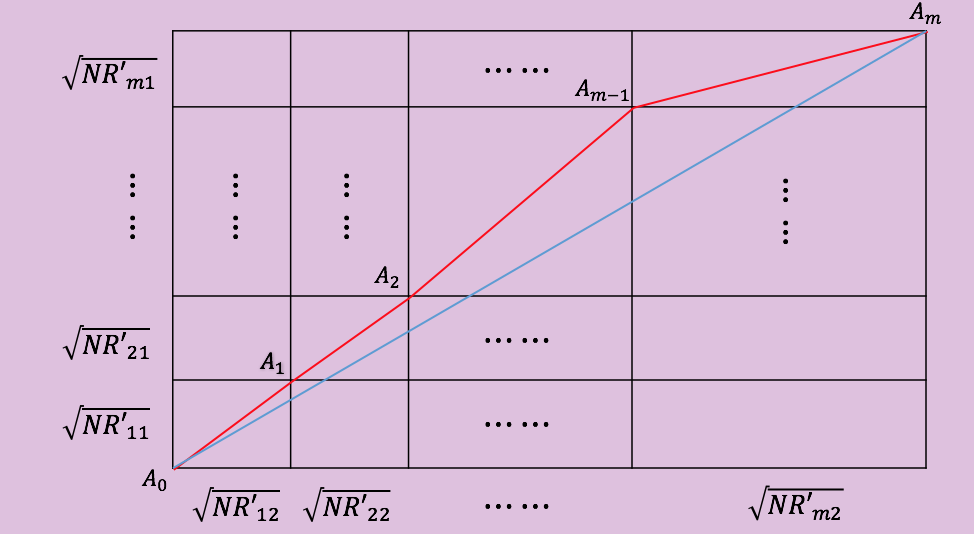
\includegraphics[width = 0.6\textwidth]{../common/m1.png}
    \begin{tikzpicture}
\pgfmathsetmacro{\HEIGHT}{1.2}
\pgfmathsetmacro{\HDOT}{2.2}
\pgfmathsetmacro{\WDOT}{3.2}
\pgfmathsetmacro{\WOne}{1.6}
\pgfmathsetmacro{\WTwo}{2.2}
\pgfmathsetmacro{\WN}{4.2}

\pgfmathsetmacro{\LEN}{\WOne + \WTwo + \WN + \WDOT}
\pgfmathsetmacro{\TH}{3*\HEIGHT+ \HDOT}

\tikzset{
  t/.style={draw, on grid, align=center, minimum height=1ex},
  coord/.style={coordinate, on grid, node distance=6mm and 25mm},
  between/.style args={#1 and #2}{
         at = ($(#1)!0.5!(#2)$)
    }
}

\draw [name path=h1] (0, 0) -- (\LEN, 0);
\draw [name path=h2] (0, \HEIGHT) -- (\LEN, \HEIGHT);
\draw [name path=h3] (0, 2*\HEIGHT) -- (\LEN, 2*\HEIGHT);
\draw [name path=h4] (0, 2*\HEIGHT + \HDOT) -- (\LEN, 2*\HEIGHT + \HDOT);
\draw [name path=h5] (0, 3*\HEIGHT + \HDOT) -- (\LEN, 3*\HEIGHT + \HDOT);

\draw[name path=v1] (0, 0) -- (0, \TH);
\draw[name path=v2] (\WOne, 0) -- (\WOne, \TH);
\draw[name path=v3] (\WOne + \WTwo, 0) -- (\WOne + \WTwo, \TH);
\draw[name path=v4] (\WOne + \WTwo + \WDOT, 0) -- (\WOne + \WTwo + \WDOT, \TH);
\draw[name path=v5] (\WOne + \WTwo + \WDOT + \WN, 0) -- (\WOne + \WTwo + \WDOT + \WN, \TH);

\path [name intersections={of=h1 and v1,by=A0}];
\path [name intersections={of=h2 and v2,by=A1}];
\path [name intersections={of=h3 and v3,by=A2}];
\path [name intersections={of=h4 and v4,by=Am1}];
\path [name intersections={of=h5 and v5,by=Am}];

\draw [red] (A0) -- (A1) -- (A2) -- (Am1) -- (Am);
\draw [blue] (A0) -- (Am);

\node [below=0.01 of A0, anchor=north east] {$A_0$};
\node [above=0.05 of A1, anchor=south east]{$A_1$};
\node [above=0.05 of A2, anchor=south east] {$A_2$};
\node [above=0.05 of Am1, anchor=south east] {$A_{m-1}$};
\node [above=0.05 of Am, anchor=south]{$A_m$};


\path [name intersections={of=h1 and v1,by=t00}];
\path [name intersections={of=h2 and v1,by=t01}];
\path [name intersections={of=h3 and v1,by=t02}];
\path [name intersections={of=h4 and v1,by=t03}];
\path [name intersections={of=h5 and v1,by=t04}];
\node [coord, between=t00 and t01] (x1){};
\node [coord, between=t01 and t02] (x2){};
\node [coord, between=t02 and t03] (x3){};
\node [coord, between=t03 and t04] (x4){};

\node [left=0.05 of x1.west] {$\sqrt{{\nr}'_{11}}$};
\node [left=0.05 of x2.west] {$\sqrt{{\nr}'_{21}}$};
\node [left=0.7 of x3.west, anchor=center] {$\vdots$};
\node [left=0.05 of x4.west] {$\sqrt{{\nr}'_{m1}}$};

\path [name intersections={of=h1 and v1,by=s00}];
\path [name intersections={of=h1 and v2,by=s01}];
\path [name intersections={of=h1 and v3,by=s02}];
\path [name intersections={of=h1 and v4,by=s03}];
\path [name intersections={of=h1 and v5,by=s04}];
\node [coord, between=s00 and s01] (y1){};
\node [coord, between=s01 and s02] (y2){};
\node [coord, between=s02 and s03] (y3){};
\node [coord, between=s03 and s04] (y4){};

\node [below=0.5 of y1.south, anchor=center] {$\sqrt{{\nr}'_{12}}$};
\node [below=0.5 of y2.south, anchor=center] {$\sqrt{{\nr}'_{22}}$};
\node [below=0.5 of y3.south, anchor=center] {$\dots$};
\node [below=0.5 of y4.south, anchor=center] {$\sqrt{{\nr}'_{m2}}$};

\node at (x1.east -| y3.north) {$\dots$};
\node at (x2.east -| y3.north) {$\dots$};
\node at (x4.east -| y3.north) {$\dots$};

\node at (y1.north |- x3.east) {$\vdots$};
\node at (y2.north |- x3.east) {$\vdots$};
\node at (y4.north |- x3.east) {$\vdots$};

\end{tikzpicture}

	 	\caption{最短路证明 \label{fig:path}}
	 \end{figure}
	 如图~\ref{fig:path},构造一个网格,其长和宽均被分成了$m$段,其第$i$段长度分别为$\sqrt{\nr'_{i1}}$和$\sqrt{\nr'_{i2}}$。

	 $S_1^{'2}+S_2^{'2}=A_0A_m^2$,即恰好等于图中蓝线的长度的平方。而
	 $$S_1^2 = (\sum_{i=1}^m \sqrt{\nr_{i1}})^2 > (\sum_{i=1}^m \sqrt{\nr'_{i1}+\nr'_{i2}})^2 = (\sum_{i=1}^m A_{i-1}A_i)^2$$
	 即所有红线长度之和的平方。根据两点之间线段最短可得$S_1^2 >S_1^{'2}+S_2^{'2}$。

	 对于拆分成$k>2$个DApp的情形,只需转化成逐次拆分然后每次应用$k=2$时的结论即可。

	 故命题得证。
\end{proof}

\subsection{推论~\ref{c1}证明}
\label{subsection:proof3}
\begin{proof}
	对于一个被$d_1$开发者收买的用户,在$d_1$进行拆分之前,可以将该用户等价于一个价值权重向量为$(1,0,0,...,0)$的正常用户。而拆分成$k$个DApp之后,假设被收买用户对这$k$个DApp的分贡献值为$\nr_{t1},...,\nr_{tk}$,其和为定值。根据特征1的证明中柯西不等式取等号的条件,可将该用户等价于一个价值权重向量为$(\sqrt{\nr_{t1}}/C,\sqrt{\nr_{t2}}/C,...,\sqrt{\nr_{tk}}/C,0,0,...,0)$的正常用户。其中$C=\sum_{j=1}^k \sqrt{\nr_{tj}}$。即对拆分出的DApp按某种比例分配权重,所有其他DApp权重为0\footnote{注意将所有价值权重同时扩大若干倍对结论没有影响,因为最终用户分贡献值总和只与权重占据的比例有关。}。此时因为
	$$\sum_{j=1}^k \sqrt{\nr_{tj}}/C =1$$
	可规约为特征2的情况,即变成满足假设的正常用户的情形。故命题得证。
\end{proof}

\subsection{性质~\ref{p3}证明}
\begin{proof}
我们先考虑某个用户将其账户拆分成两个子账户的情况。固定其他用户的行为,假设$c$为该用户原账户,$a$,$b$为拆分后子账户。$S,S'$分别为拆分前后该用户指定DApp的排名分。$U,U'$分别为拆分前该用户。根据定义,有
$$S= \sqrt{\nr_c}+O,~~S'=\sqrt{\nr_a}+\sqrt{\nr_b}+O$$
其中$O$为其他用户对该DApp的贡献值之和,是个定值。

由~\ref{eq:sqrt_nr}可得$S < S'$,即该DApp排名分不会增加。

同时,根据定义有
$$U = \frac{S}{S+P}\lambda M,~~U' = \frac{S'}{S'+P} \lambda M$$
其中$P$为其他DApp的排名分的平方和,是个定值,故
$$U \geq U' \Leftrightarrow S \geq S'$$
由$S < S' $可得 $U \leq U'$,即该DApp最终奖励不会增加。
\end{proof}